% !TeX spellcheck = <none>
\documentclass[./\jobname.tex]{subfiles}

\begin{document}
\definecolor{light-gray}{gray}{0.9}

\chapter{Task Description}

This project is about constructing and building a 3-axis robot. The robot is equipped with two cameras and a red laser-pointer. The user can take a green laser-pointer to direct the robot into a different position. In order to avoid permanent sight-damage, the robot should avoid shining the laser into faces of surrounding humans. The following list contains the main working steps:

\begin{itemize}
	\item design and construct the 3-axis robot 
	\item manufacture and assemble the robot parts 
	\item develop the backwards kinematic 
	\item implement the backwards kinematic in C and compile to DLL 
	\item find green laser point in 3D stereo image with OpenCV in Python 
	\item drive the red laser point of the robot to the green laser point of the human
	\item planned but optional: 
	\begin{itemize}
		\item plan path from current position to green laser position 
		\item implement controller to correct deviance between red and green laser point 
		\item avoid human faces along the way
	\end{itemize}
	
\end{itemize}


\chapter{Design}

The robot consists of 3 Dynamixel MX-64AT motors, 2 Microsoft HD 3000 lifecam and a laser module DB635-1-3-FA(14x45)-ADJ from Picotronic. Aluminium frames are attached to the motors to build the framework of the robot. The cameras and laser-pointer are connected with aluminium brackets to the robot. The design of the robot and its components is established with SolidWords. The whole robot is mounted on aluminium profiles to improve the handling and to store of the electrical hardware. Beside the cables, a power supply for the motors and laser pointer, an emergency stop button and communication components for the motors are required. The cameras are directly connected to the laptop or computer via the USB ports. This means that the laptop requires 3 USB sockets. A connection via a USB-Hub failed as the OpenCV library could not find the cameras. \\
The table \ref{tab:camera_before_after} shows how the cameras were modified in order to properly attach them to the robot tool. \\
The table \ref{tab:3d_rander} displays a 3D render of the completely assembled robot.\\
Finally, the finished robot can be seen in figure \ref{fig:final_assemgly}

\begin{table}[H]
	\centering
	\noindent\adjustbox{max width=\linewidth}{
		\begin{tabular}{c c}
			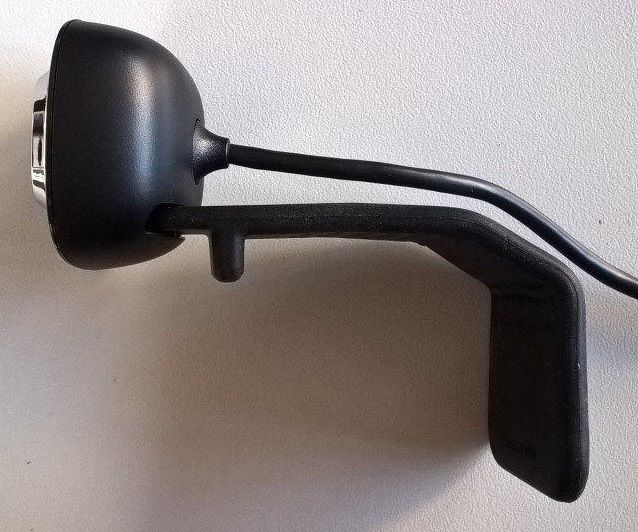
\includegraphics[width=0.6\textwidth]{img/foto/camera_with_stand.jpg}
			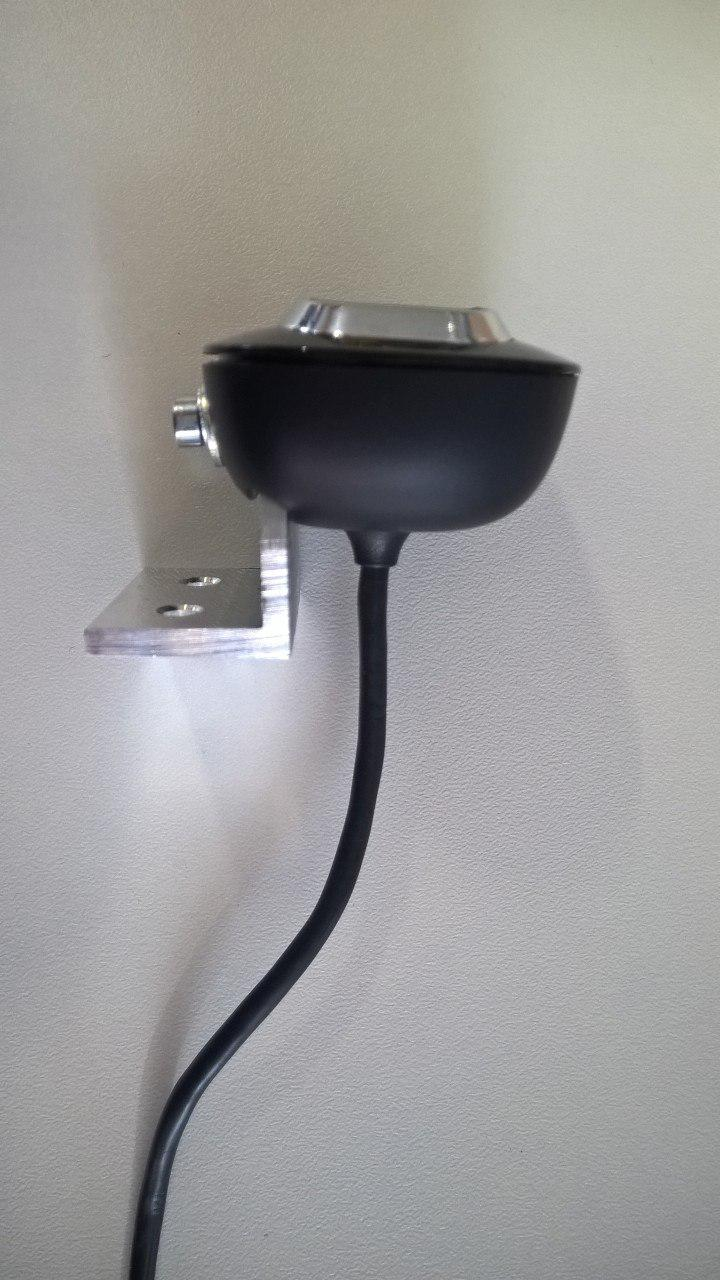
\includegraphics[width=0.49\textwidth]{img/foto/camera_without_stand.jpg}
		\end{tabular}
	}
	\unterschrift{comparison of the cameras before and after modification}{}{}
	\label{tab:camera_before_after}
\end{table}


\begin{table}[H]
	\centering
	\noindent\adjustbox{max width=\linewidth}{
		\begin{tabular}{c c}
			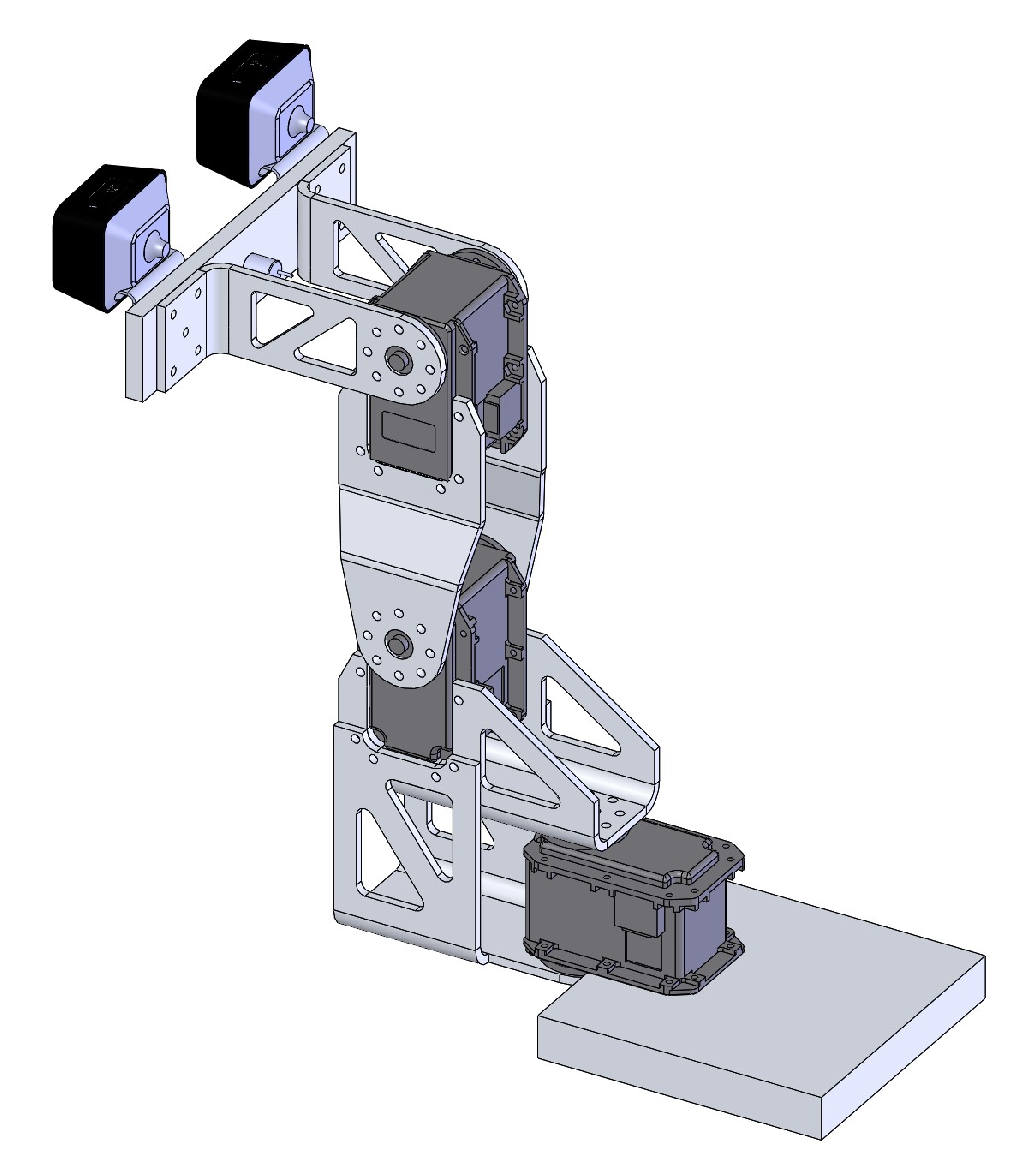
\includegraphics[width=0.75\textwidth]{../img/pdf/robot_3d_side.pdf}
			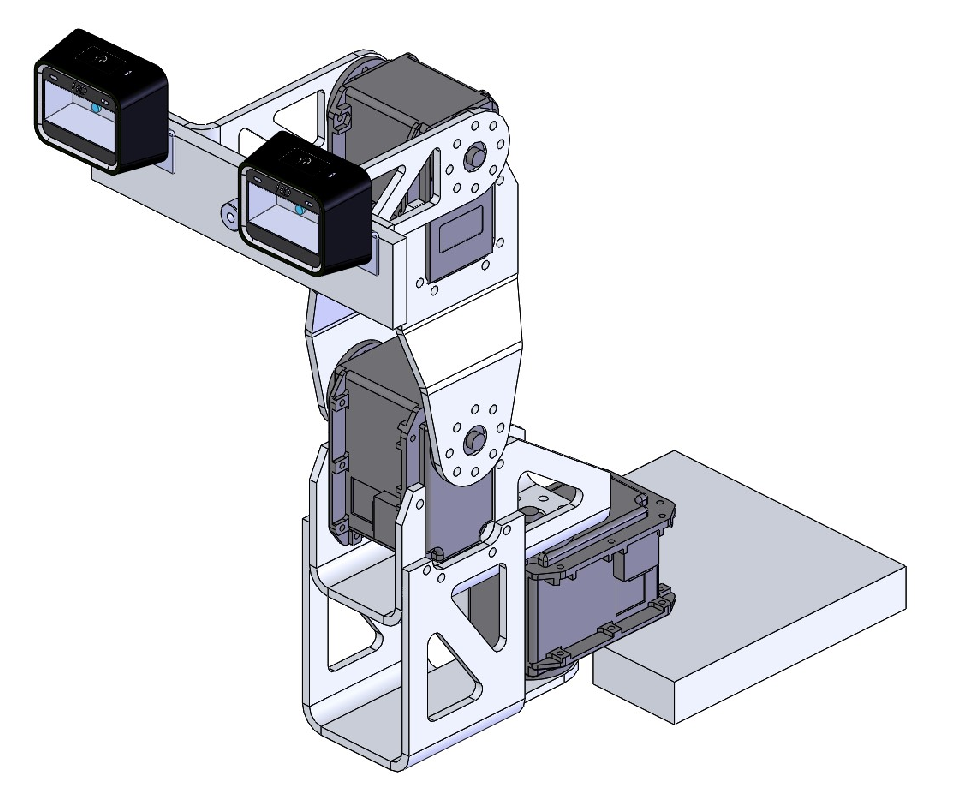
\includegraphics[width=1\textwidth]{../img/pdf/robot_3d_front.pdf}
		\end{tabular}
	}
	\unterschrift{3D render of the assembled robot in SolidWorks}{}{}
	\label{tab:3d_rander}
\end{table}



\begin{figure}[H]
	\centering
	\noindent\adjustbox{max width=\linewidth}{
		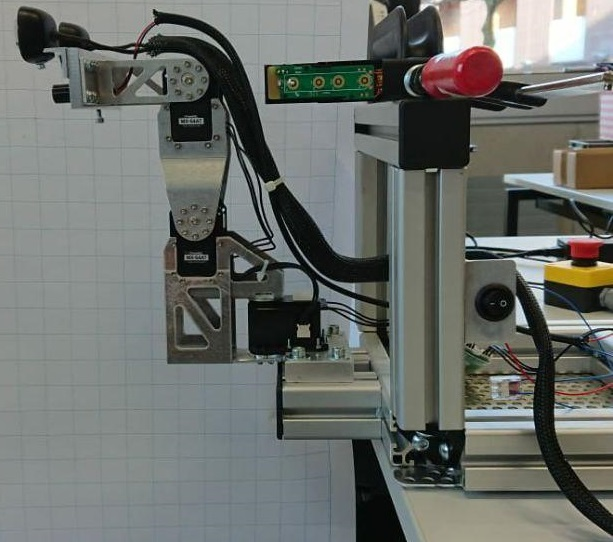
\includegraphics[width=0.8\textwidth]{img/foto/final_robot_photo.jpg}
	}
	\unterschrift{final assembly of the robot}{}{}
	\label{fig:final_assemgly}
\end{figure}


\chapter{Calculation}
This chapter describes the mathematical formulations that are needed to control the robot. This includes the backwards kinematics as well as the formulas for setting $\theta_{0,1,2}$. 

\section{Backwards Kinematic}

The following figure \ref{fig:robot_coord} shows the coordinate systems that are used to get the link parameters shown in table \ref{tab:link_params} below. The link parameters are established using the Deviant Hartenberg convention mentioned in \cite[p. 70- 79]{Craig2018}.

With the knowledge of the link parameters, the transformation matrices are generated in the next step. The full matrix can be seen in equation \ref{eq:transformationmatrix}

\begin{figure}[H]
	\centering
	\noindent\adjustbox{max width=\linewidth}{
		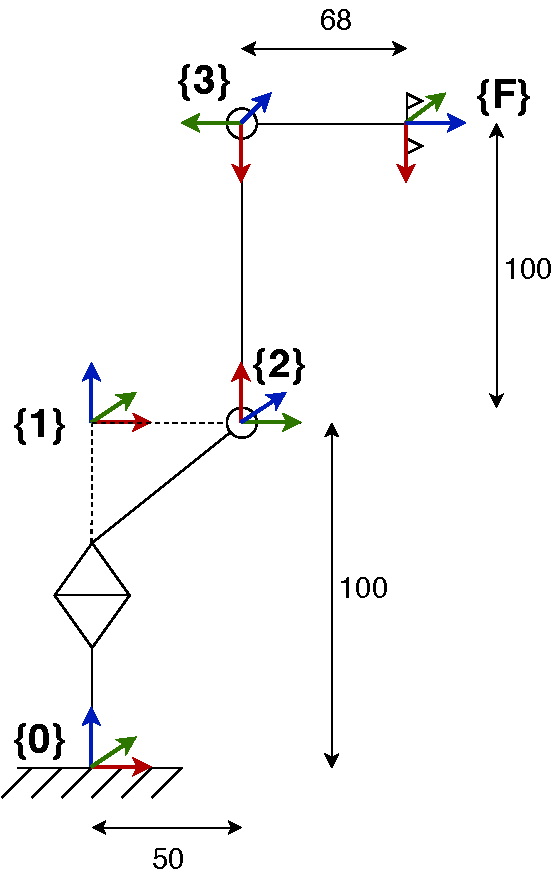
\includegraphics[width=0.4\textwidth]{img/pdf/robot_axis_coord.pdf}
	}
	\unterschrift{robot axis coordinate systems used to calculate the link parameters}{}{}
	\label{fig:robot_coord}
\end{figure}





\begin{table}[H]
	\centering
	\noindent\adjustbox{max width=\linewidth}{
		\begin{tabular}{|c|c|c|c|c|}
			\hline
			$i$ & $\alpha_{i-1}$ & $a_{i-1}$ & $d_i$ & $\theta_{i-1}$\\ 
			\hline
			1 & 0 & 0 & 100 & $\theta_0$\\  
			2 & -90 & 50 & 0 & $\theta_1 - 90$\\ 
			3 & 0 & 100 & 0 & $\theta_2 + 180$\\ 
			F & 90 & 0 & 68 & $0$ \\
			\hline
		\end{tabular}
	}
	\unterschrift{table of link parameters}{}{}
	\label{tab:link_params}
\end{table}



\begin{equation}
\label{eq:transformationmatrix}
\begin{split}
& T =  \\
& \begin{bmatrix}
-c0c1s2 -c0c2s1 & -s0 & c0c1c2 - c0s1s2 & a2c0 + dF (c0c1c2 - c0s1s2) + a3c0s1 \\
-c1s0s2 -c2s0s1 &  c0 & c1c2s0 - s0s1s2 & a2s0 + dF (c1c2s0 - s0s1s2) + a3s0s1 \\
s1s2 - c1c2     &   0 & -c1s2 - c2s1 & d1 + a3c1 + dF(-c1s2 - c2s1) \\
0               &   0 & 0 & 1 \\
\end{bmatrix}\\
\end{split}
\end{equation}


\subsection{Implementation}
For controlling the robot, several functions are written in C and compiled to a DLL. The functions are built on the Dynamixel library \cite{Robotis2019}. The DLL provides the following methods: 
\begin{itemize}
	\item \colorbox{light-gray}{\lstinline[basicstyle=\ttfamily\color{black}]|int robot_start();|} \\
	Sets up the communication with the robot by returning the port number. This number must be provided in every other function. Further this function sets up the main parameters of every motor like the velocity limits.
	\item \colorbox{light-gray}{\lstinline[basicstyle=\ttfamily\color{black}]|void robot_stop(int port_num);|} \\ 
	Stops the robot by driving to the home position and freeing the device with the port number. 
	\item \colorbox{light-gray}{\lstinline[basicstyle=\ttfamily\color{black}]|void robot_home(int port_num);|} \\
	Separate function for driving the robot to the home position. 
	\item \colorbox{light-gray}{\lstinline[basicstyle=\ttfamily\color{black}]|int robot_drive(float z, float alpha, float beta, int port_num);|} \\
	Tells the robot to drive to a specific position specified by $\alpha$, $\beta$ and z. The motion towards this position is not planned. 
	\item \colorbox{light-gray}{\lstinline[basicstyle=\ttfamily\color{black}]|int robot_reached_target(float z, float alpha, float beta, \ \ \ \ \ int port_num);|} \\
	This function checks if the robot is at the specified $\alpha$, $\beta$ and z position and returns 1 if it reached the target (otherwise 0).
	\item \colorbox{light-gray}{\lstinline[basicstyle=\ttfamily\color{black}]|void robot_set_theta(float theta0, float theta1, float theta2, \ \ \ \ \ int port_num);|} \\
	Instead of specifying a global position, this function allows to set the axis angle $\theta$ by its own. 
	\item \colorbox{light-gray}{\lstinline[basicstyle=\ttfamily\color{black}]|float robot_get_theta0(int port_num);|} \\
	Returns the angle $\theta_0$ that the robot is at that time.
	\item \colorbox{light-gray}{\lstinline[basicstyle=\ttfamily\color{black}]|float robot_get_theta1(int port_num);|} \\
	Returns the angle $\theta_1$ that the robot is at that time.
	\item \colorbox{light-gray}{\lstinline[basicstyle=\ttfamily\color{black}]|float robot_get_theta2(int port_num);|} \\ 
	Returns the angle $\theta_2$ that the robot is at that time.
\end{itemize}
The functions \textit{robot\textunderscore drive} as well as the function \textit{robot\textunderscore set\textunderscore theta} are non-blocking. This means that the function returns, before the robot reached the target. Blocking functions can be easily created outside the DLL by simply polling the functions \textit{robot\textunderscore reached\textunderscore target} or \textit{robot\textunderscore get\textunderscore theta}.  



\section{Goal Robot Configuration}
\label{sec:calc_robot_config}

The laser point on the wall can be described by only to 2 DOF, vertical and horizontal coordinates. To track the laser point, the robot has to change 2 DOF likewise. Even though the robot has 3 rotation axis, it only satisfy 2 DOF, because $theta_1$ and $theta_2$ directly depend to each other. Therefore, one of these angles can be set to any arbitrary angle. In this case $theta_1$ is constantly set to 0°. With the 2 cameras and the knowledge of the transformation matrices of the robot, the vertical and horizontal coordinates of the laser point are received and transformed into 3D coordinates of the robot base coordinate system.

As a result, the rotation angle of the motors can be calculated. $\theta_0$ is a simple geometric problem and can be easily calculated with trigonometric functions (see figure \ref{fig:3d_point_base}). The equation \ref{eq:theta_2} for $\theta_2$ is slightly more advanced. Additionally, the length and height of the robot components have to be taken in consideration.

\begin{figure}[H]
	\centering
	\noindent\adjustbox{max width=\linewidth}{
		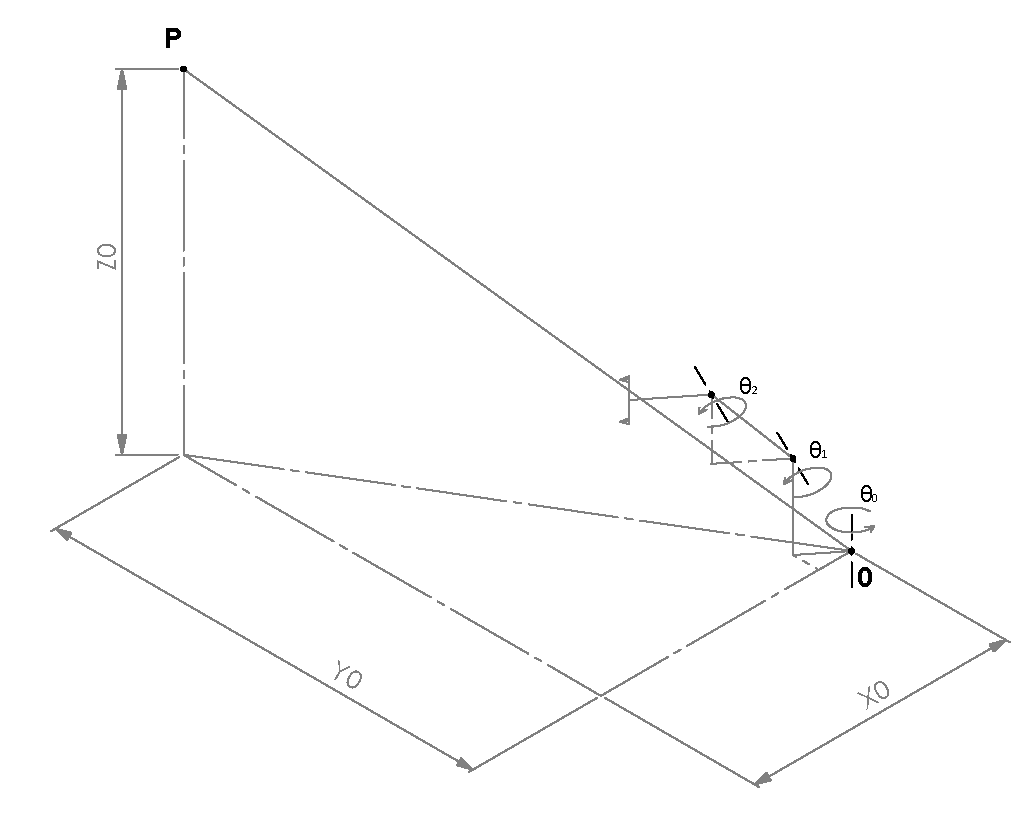
\includegraphics[width=0.8\textwidth]{img/pdf/robot_3d_point_base.pdf}
	}
	\unterschrift{camera calibration app flowchart}{}{}
	\label{fig:3d_point_base}
\end{figure}

\begin{equation}
\label{eq:theta_0}
\theta_0 = arctan \left( \frac{Y_0}{X_0} \right) 
\end{equation}

\begin{equation}
\label{eq:theta_2}
\theta_2 = -1 \cdot arctan \left( \frac{ Z_0 - 100 - 100 cos(\theta_1)}{\sqrt{X_{0}^{2} + Y_{0}^{2}} - 50 - 100 sin(\theta_1)} \right)
\end{equation}

\chapter{Stereo Vision}

The idea of this project is to drive directly to the correct point, without using a closed loop controller of any sort. This is done by measuring the 3D point with a stereo camera and calculating back to the desired robot configuration (as shown in \ref{sec:calc_robot_config}). In order to measure the correct point, the cameras need to be calibrated. Further, a reliable method for finding the laser-point is needed. All vision related tasks are done with \cite{2014opencv}

\section{Camera Calibration}
At first a camera calibration application is written, that allows to take images, calculate the two single camera matrices and estimates the translation and rotation between the two cameras. The flowchart in figure \ref{fig:cam_cal_app_flowchart} shows the main outline of the camera calibration app. 

Three quality measures are deployed to verify that the matrices are correct: 
\begin{itemize}
	\item measuring a known 3D structure with the calibrated stereo camera tool
	\item using the same pictures of the chessboard in MATLAB and comparing the calculated matrices
	\item plausibility check for the translation vector and the rotation matrix between the cameras
\end{itemize}

Besides the camera calibration towards each other, the main camera (left) must also be calibrated to the TCP. This is called the hand-eye calibration. The following matrix \ref{eq:HE} shows the hand-eye calibration. Although there are more complex methods to generate this transformation matrix, it can also be measured from the real tool. The figure \ref{fig:hand_eye_coord} shows the rotation between the TCP coordinate system and the camera coordinate system.

\begin{equation}
\label{eq:HE}
HE = 
\begin{bmatrix}
0.0  & 1.0 & 0.0 & -28.5 \\ 
-1.0 & 0.0 & 0.0 & 45.0 \\
0.0  & 0.0 & 1.0 & 28.0 \\ 
0.0  & 0.0 & 0.0 & 1.0 \\
\end{bmatrix}
\end{equation}

\begin{figure}[h]
	\centering
	\noindent\adjustbox{max width=\linewidth}{
		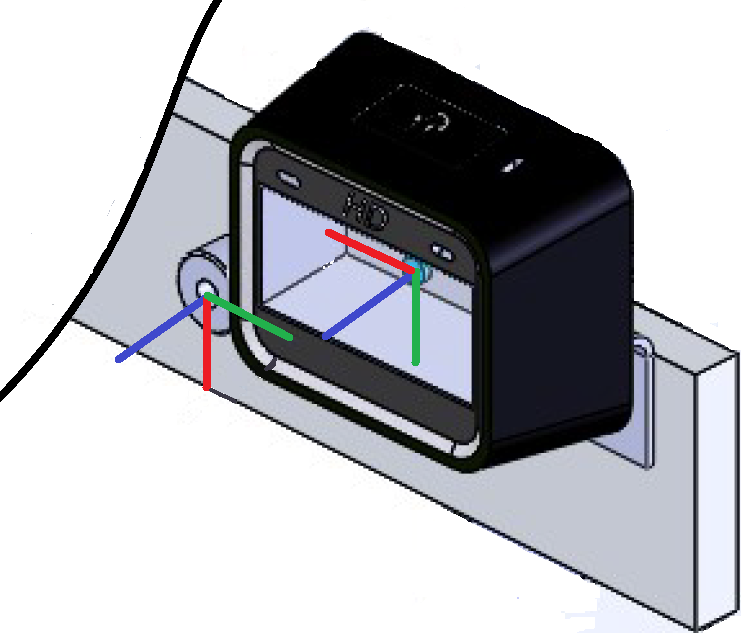
\includegraphics[width=0.4\textwidth]{img/png/hand_eye_coord.png}
	}
	\unterschrift{hand-eye coordinate system transformation}{}{}
	\label{fig:hand_eye_coord}
\end{figure}

\begin{figure}[h]
	\centering
	\noindent\adjustbox{max width=\linewidth}{
		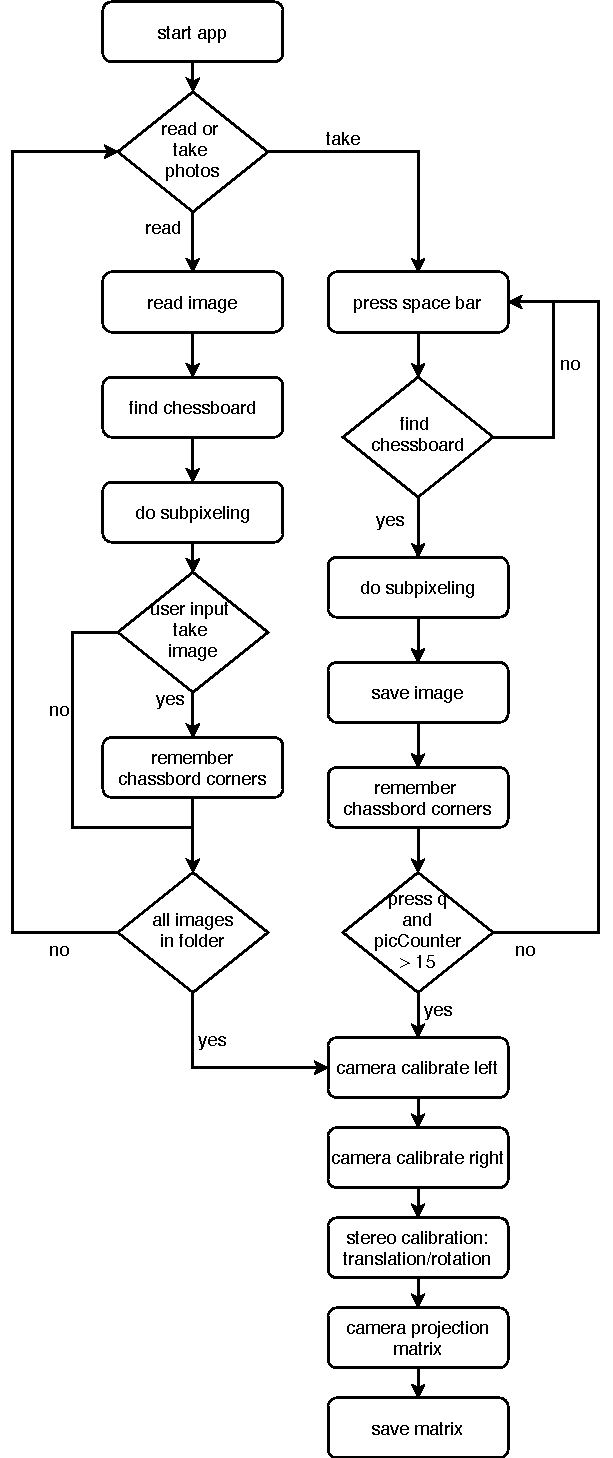
\includegraphics[width=0.6\textwidth]{img/pdf/camera_calibration_app_flowchart.pdf}
	}
	\unterschrift{camera calibration app flowchart}{}{}
	\label{fig:cam_cal_app_flowchart}
\end{figure}

\section{Laser Point Detection}
The second part is about detecting the laser point in an image. To make the task simpler, the laser point may only be projected onto a white flip board chart. \\
Two methods for detecting the laser point are tested. 

\subsection{Method 1: HSV Threshold}
As lasers are monochromatic one could think about looking for a certain colour. The idea is to define a threshold in HSV-colour space and only look at the pixels that are within this band. By applying a dilation function to the binary image, the weakly connected pixels are morphed together and form blobs. Then the function \textit{findCountours} is deployed to detect the connected areas of white pixels. Finally, the first (biggest) area contour is taken and the centre of mass is calculated. This is the 2D point in one image. \\
This method did not work very well. Some problems have been identified: 
\begin{itemize}
	\item Taking the biggest area is not very sensible. More constraints could be helpful like: size threshold, convexity or previous point.
	\item As the automatic mode of the camera is not deactivated the colour of the laser point might change with different lighting scenarios. 
	\item The definition of the colour threshold is not trivial: Either too many pixels or too few are taken. Especially with a colourful surrounding this trade-off is hard to control. 
\end{itemize}

\subsection{Method 2: Template Matching}

The second method uses template matching to find the green laser point. The process outline as follows: a template slides over the image and at every pixel they are compared. The comparison results a scalar value which are then stacked together to create something like a `heat-map'. The larger the scalar is at an index, the better is the correspondence between the image and the template. \\
There are many different methods for comparing two images defined in OpenCV. The utilize method was found to work best for this sort of object detection. The formula is shown in equation \ref{eq:template_matching}. \\
The templates are created before every run. In order to make that process as user-friendly as possible, a GUI based configuration app is created. The templates can be seen in the table \ref{tab:laser_template_comp}. \\
The main characteristics of this method are: 
\begin{itemize}
	\item This method works much better with different lighting scenarios than the HSV-threshold.
	\item Motion blurring results in an unstable detection of the laser point. Thus, fast movements with the robot and by hand should be avoided. 
	\item Whenever there is no green laser point in the image, the red laser is detected as green, since this is now the best match. 
	\item This method only works with the background (e.g. white flip board) specified in the template. 
\end{itemize} 

\begin{equation}
R(x,y) = \frac{\sum_{x',y'} (T'(x',y') \cdot I'(x + x', y + y'))}{\sqrt{\sum_{x',y'} T'(x',y')^{2} \cdot \sum_{x',y'} I'(x + x', y + y')^{2}}}
\label{eq:template_matching}
\end{equation}


\begin{table}[h]
	\centering
	\noindent\adjustbox{max width=\linewidth}{
		\begin{tabular}{c c}
			
\includegraphics[width=0.295\textwidth]{img/png/green_laser_template.png}
			
\includegraphics[width=0.3\textwidth]{img/png/red_laser_template.png}
		\end{tabular}
	}
	\unterschrift{laser point template as created by the configuration app}{}{}
	\label{tab:laser_template_comp}
\end{table}


\chapter{Main App}
This chapter describes the algorithmic steps taken in the main application as seen in the flowchart \ref{fig:main_app_flowchart}. The action \textit{transform 3D point to robot base} consists of multiple steps itself: 

\begin{itemize}
	\item Multiply the 3D point with the hand-eye calibration to transform the point into the TCP frame, as seen in \ref{eq:HE} 
	\item Transform the point to the robot base coordinate system by multiplying with the backwards kinematic in \ref{eq:transformationmatrix}. 
\end{itemize}

\begin{figure}[h]
	\centering
	\noindent\adjustbox{max width=\linewidth}{
		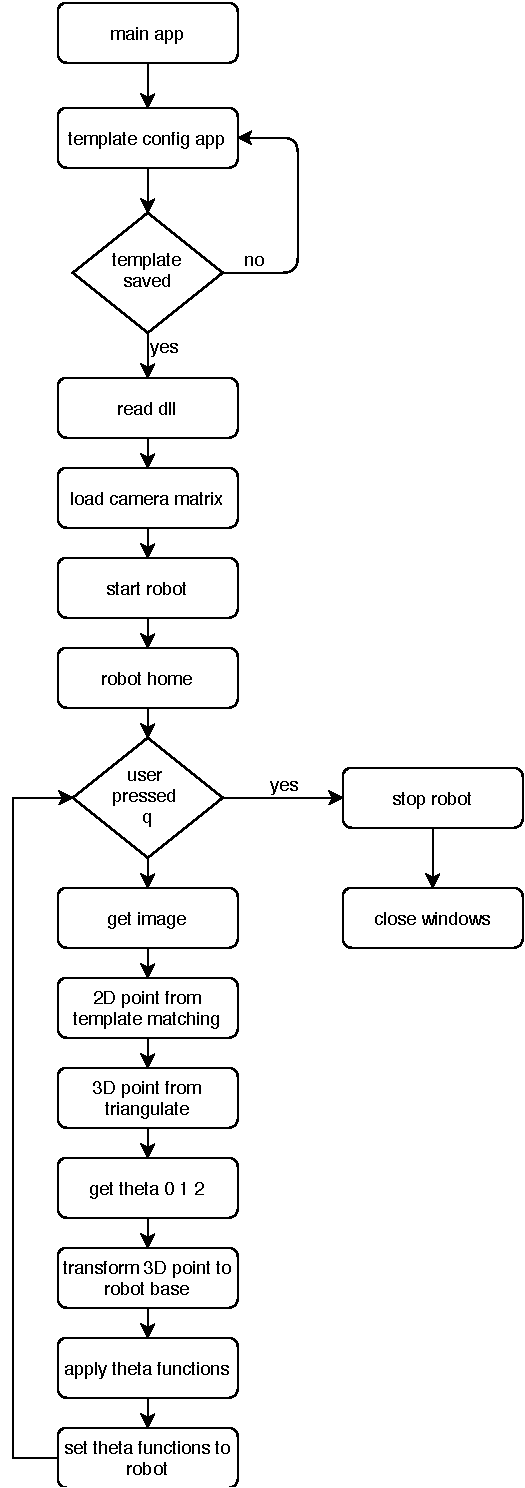
\includegraphics[width=0.5\textwidth]{img/pdf/main_app_flowchart.pdf}
	}
	\unterschrift{camera calibration app flowchart}{}{}
	\label{fig:main_app_flowchart}
\end{figure}


\chapter{Conclusion}

We find, that template matching method is better suited to detect small objects in a constantly changing image rather than searching the images for a specific colour.

The resting distance between green and red laser point, as seen in figure \ref{fig:resting_offset} results from the offset of the laser pointer to the robot tool centre. That can be easily adjusted with a new bracket. To avoid any systematic errors, the laser pointer has to be mounted colinear with the z-axis of the robot tool.  

Another current problem is the high energy consumption of the laser pointer. Within a half an hour, the intensity of the laser pointer dropped significantly. In the next step, a more appropriate power supply should be installed.

An additional option could be to specify $theta_1$ as a variable instead of a constant and find a more advanced system of equations.   

\begin{figure}[H]
	\centering
	\noindent\adjustbox{max width=\linewidth}{
		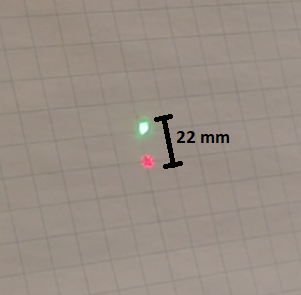
\includegraphics[width=0.5\textwidth]{img/foto/resting_ofset.png}
	}
	\unterschrift{resting offset between laser points}{}{}
	\label{fig:resting_offset}
\end{figure}


\end{document}
